\section{Background}
In this section, we first introduce the brief background, including virtualization and RDMA. 

\subsection{Cloud and Virtualization}
Cloud is popular for its efficiency and elasticity, and virtualization is the basic for clouds. Nowadays, VMs and containers are both common virtual instances in clouds. VMs need emulate whole virtual hardware environments for guest operation system with hypervisor (kernel-space). So, applications in VMs is isolated by guest OS with more security but higher overhead. Containers are shared with the host OS but with runtime isolation. So, containers have low overhead and fast boot-up time.

For software virtualization of I/O devices, there are two main choices for where to emulate the device: kernel-space and user-space. In kernel-space, the codes of device emulation are inserted into hypervisor or host kernel. Compared to kernel-space, there are three advantages for user-space: first, the attack surface is limited for user-space with minimal inserted code into kernel/hypervisor; second, managment development is flexible in user-space; third, the inserted codes are often depenedent on hardware-specific APIs (e.g. OS architecture, device driver). For example, vhost-net~\cite{vhost-net} is the kernel-space network device and vhost-user-net~\cite{vhost-user-net} has user-mode virtual device. 

\begin{figure}[!ht]
\centering
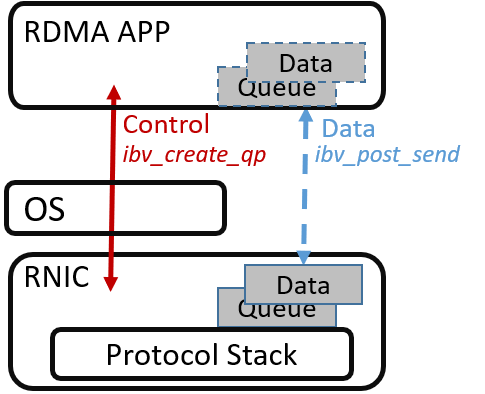
\includegraphics[width=0.6\linewidth]{images/rdma-feat.png}
\caption{Native RDMA Feature}
\label{fig:rdma-feat}
\end{figure}

\subsection{RDMA}
As popular high-performance network in supercomputing, RDMA has hardware protocol stack and zero copy technology. With RDMA, applications can bypass the kernel to read and write remote memory data, without the participation of remote CPU. 

Verbs~\cite{verbs} is the basic interface for applications to utilize RDMA. It is similar as socket for traditional network applications. As shown in Figure~\ref{fig:rdma-feat}, RDMA Verbs is separate to control path and data path to achive high-performance. In control path: applications open device and manage RDMA resources. The main RDMA resources include Queue Pairs (QPs), Complete Queues(CQs), Memory Regions (MRs). The control verbs include ibv\_create\_qp, reg\_mr;  In data path: applications use RDMA resources to transport data. The data verbs include ibv\_post\_send and ibv\_post\_recv. Compared control path, data path bypasses the kernel to avoid context switch.

In a RDMA workflow, the communication is based on Queue Pair (QP). The application writes the RDMA work request to the QP, and then ``press''  the RNIC's doorbell register, which is mapped to application when context init, and the RNIC's hardware processor will execute the work request in the QP to forward data. There are two modes for RDMA connect-based communication: one-sided and two-sided. One-sided is that remote server is awareness when client reads or writes its registered memory; Two-sided is that one sends messages after the peer is ready to receive.
